\chapter{Post-editing profiles -- which competences are needed?}\label{sec:9}

    \objectives{
     You will learn...
        \begin{itemize}
            \item which competences are important for MT and PE,
            \item which job profiles might be interesting in the field of PE,
            \item what is necessary for training.
        \end{itemize}
     }


\section{PE competences}\label{sec:9:1}

Many aspects have to be considered when dealing with MT and PE. Post-editing is a complex task. Accordingly, a qualified post-editor needs specific competences to be able to fulfil all the requirements of such a task. The proposed PE competence model (\figref{fig:key:9:1}) is a further development of \citet{nitzke2019risk} based on PACTE’s (\citeyear{beeby2003building}) translation competence model and the revision competence model by \citet{robert2017towards} since they share some of the competences needed for post-editing MT output. The differences and commonalities will be explained in the following. Further, not all decisions are necessarily made by the client – some clients might need a lot of guidance when it comes to MT. A post-editor, therefore, must be able to make informed decisions concerning risk assessment as well as the integration of MT and PE in the translation workflow.

\begin{figure} 
% 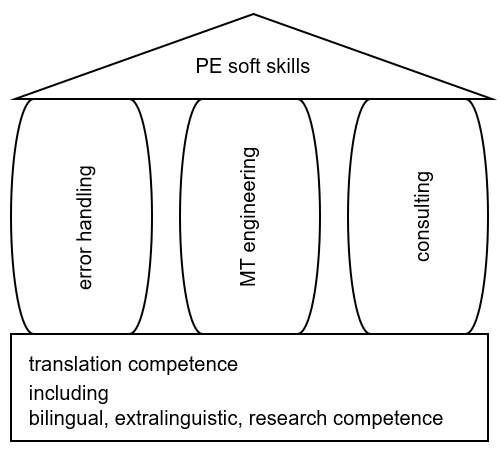
\includegraphics[height=0.3\textheight]{figures/Competence Model.PNG}
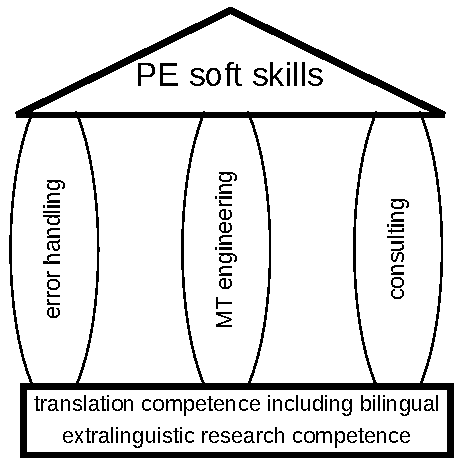
\includegraphics[height=0.3\textheight]{figures/jobprofile0.pdf}
\caption{PE competence model}
\label{fig:key:9:1}
\end{figure}

If we consider the competence model as a house of PE competences, the architecture of the house is grounded on the basic competences we also expect from professional translators: translation competences, including bilingual, extralinguistic and research competence. This is also the basis for a skilled post-editor. Translation competences have been described in different models over the years, e.g., PACTE (\citeyear{beeby2003building}), \citet{emt2009competences}, \citet{gopferich2009towards}. It is essential that post-editors are skilled translators, because they need the same basic skill set. These skills include amongst others knowledge about text type conventions, the ability to deal with style guides or controlled languages, knowledge about contrastive differences, cultural specificities, etc. As they automatically learn from data, the machines might be able to recreate some text type conventions or cultural differences, but, accordingly, the training data have to be very good and specific. Nonetheless, chances are high that the machine will make mistakes, especially in these areas. Hence, a professional translator is needed to post-edit the machine-translated output, especially when the goal is a high quality target text.

Similar to translation and revision competence, a post-editor has to have proficient knowledge of the source and target language, as monolingual PE always bears the risk that content mistakes are not recognised (see \sectref{sec:4:1:3}). This basic competence is often referred to as bilingual competence in translation competence models.

Another similarity to specialised translation and revision tasks is that a post-editor also needs to have general world knowledge as well as the relevant domain knowledge in order to properly understand the thematic subject of the source text. This knowledge can be summarised with the term extralinguistic competence. Knowledge about cultural domain differences helps the post-editor to interpret the meaning in the source text correctly and transfer it adequately to the target text.

Finally, a post-editor also needs to know where and how to find information he or she does not have, i.e. research competence is required. Depending on the thematic field of the translation, specialised (online) dictionaries might be the first choice, whereas, for others, parallel corpora or thesauri might be better options. Efficient research strategies positively influence the workflow time of a PE task. Further, the post-editor needs to learn to what extent he or she can trust the MT output, e.g. concerning the correct translation of terminology, and when MT decisions have to be changed.

\bigskip

The three pillars of the model define the additional competences: error handling, which includes error spotting, error classification, and error correction; MT engineering, which includes training and assessment of MT systems, and specialised consulting competences, which are tailored to the needs of post-editing jobs. Let us have a closer look at these competences, which will be used to describe different job profiles later in \sectref{sec:9:2}.

Let us first discuss the error-spotting competence. Different MT systems (rule-based, statistical, neural, etc.) generate different errors. Hence, it is important to know what kind of system will be used and to have knowledge of the approach used in the MT system. In recent years, neural MT has become the state-of-the-art. However, it is still plausible that statistical or hybrid systems will be used -- or that other MT approaches will be developed in the future. However, let us focus briefly on neural MT systems. Many errors generated by neural MT systems are more difficult to identify compared to statistical MT since the MT output is more fluent and seems to be correct, which leads to the problem of overlooking mistakes that are not obvious (\citealt{toral2018post}, e.g., show that pauses become fewer but longer when post-editing neural MT output). Therefore, the post-editor has to be trained to spot exactly these more fine-grained mistakes and problems. Further, the post-editor has to work efficiently and has to know which errors have to be corrected to which extent according to the respective guidelines. This means that the trained post-editor should be able to identify what kind of mistake (s)he stumbled across and whether this mistake has to be improved or not according to the job-specific guidelines in order to avoid over-corrections or over-editing (see e.g. \citealt{nitzke2020preferential} and \citealt{vardaro2019translation}). For example, different studies have shown that post-editors are primed by the MT output (e.g. \citealt{bangalore2015role}) or at least feel primed by the MT output (e.g. \citealt{moorkens2018translators}). Post-editors should be aware of these phenomena, should be able to recognise them, and should know how to deal with them. 

A post-editor needs some knowledge about machine translation engineering, although the depth of knowledge might vary across the different job profiles (see \sectref{sec:9:2}). As we have already mentioned, the different MT systems generate different problems and mistakes. Hence, a post-editor needs to know how an MT system works and which possible pitfalls it may generate. MT systems often generate other problems than human translators produce (\citealt{carl_post-editing_2015}, \citealt{nitzke2019problem}). Most of them are related to the architecture of the MT system. Knowing how MT is implemented helps to spot potential problems or difficulties. Ideally, in our view, a post-editor should be able to assess the quality of the MT training materials and even to improve the training process if necessary. Some post-editors might even help to set up a new system as they can gather and evaluate the training data.

Finally, a certain consulting competence is essential. Many clients might not be aware of the pros and cons of using machine translation systems for the translation process. Even clients that often work with translation professionals and language service providers might not be aware of risks and strategic processes as PE has only recently become established on the market. Hence, a post-editor has to inform the customer or project manager about potential risks as well as problem-solving strategies, respectively, i.e. the risk assessment should enable the post-editor to give advice on these questions, even if the post-editor is not fully responsible for the decisions regarding the overall project. A post-editor should be able to voice his/her concern if a decision seems too risky or suggest the use an MT system if it seems plausible for the job to avoid regret in hindsight. This kind of support should also be included in price calculations.   
The consulting competence goes hand in hand with risk assessment and service competences that are part of what we call PE soft skills. The risk assessment competence is very important for judging the project and supporting the client, as already discussed in \sectref{sec:7} and \sectref{sec:8}. Depending on the position of the post-editor in the whole PE process, the post-editor might be more or less responsible for the decisions concerning the use of MT. However, every post-editor should have at least little knowledge about potential risks associated with using MT systems in the PE process in order to support the clients and raise doubts if certain decisions seem risky or implausible (\citealt{kenny2020fair}).
In the field of PE, service competence means that the post-editor should be able to calculate prices competently, consciously, and transparently considering the quality of the MT output and the necessary PE effort, even though measuring and estimating PE effort is challenging (there has been a lot of research in this area, see e.g. \citealt{specia2011exploiting}; \citealt{moorkens2015correlations}; \citealt{schaeffer2014measuring}). However, it should become easier to predict the PE effort with increasing experience. Further, as the market is still developing, professional associations will be able to give more information on this topic in the future, which will facilitate a career entry. Another aspect of this competence includes handling state-of-the-art CAT and revision tools as well as integrated MT systems. The post-editor must be able to post-edit the texts efficiently according to the client’s guidelines and must be able to adapt to the client's quality expectations. Best practice would be to immediately save the post-edited or finally revised text in the TM or in the training database.

In summary, the post-editor should know the translation market, including all aspects of MT and PE, and should be able to negotiate with the customer on an equal footing. The post-editor should be able to match the needs of the customer with the set-up and conditions of the PE task as well as with the resources available to be able to make an appropriate offer that calculates a realistic time and cost frame for the job.

\bigskip

In our house of PE competence, the three pillars are framed by a roof, which represents soft skills for post-editors. As described in a similar way in the models by PACTE (\citeyear{beeby2003building}) and \citet{robert2017towards}, a PE task is also influenced by its surrounding factors such as:

\begin{itemize}
 \item psycho-physiological components, 
 \item an affinity towards the latest technological developments,
 \item the PE brief including guidelines for the PE task,
 \item the post-editor’s self-perception.
\end{itemize}{}

Some of the psycho-physiological components are especially important for post-editors, such as a well-developed ability to concentrate and sustain attention (especially in the case of repeated mistakes in the MT output), stress-resistance, logical reasoning, analytical thinking, and quick-wittedness. An affinity to working with the latest technological developments is an essential requirement to work as a post-editor, because PE tasks always go hand in hand with MT and CAT tools.

A PE job can only be accomplished successfully if the post-editor knows the target audience, the skopos of the target text, the effort that needs to go into the PE task (light vs. full PE, etc., see \sectref{sec:4}), which should all be summarised in a PE brief. Further, it has to be obvious which the post-editor's responsibilities are (e.g. maintaining of the translation memory and terminology management systems, reporting or even correcting flaws of the MT system).

\hspace*{-3pt}The broader perspective of the role and responsibilities of the post-editor should be accompanied by a new self-perception and appropriate professional ethics. When the market began to change, translators perceived PE as a mediocre task for quite a while \citep{guerberof2013professional}. However, post-editors should perceive themselves not only as mere proof-readers of MT output, but as competent language consultants and experts in creating PE processes to establish PE as a professional task in its own right. As such, they should take responsibility for the successful creation of the target text. It also requires new professional ethics that still need to be conceptualised. The new ethos should incorporate elements such as the willingness of post-editors to accept that sometimes the quality of the target text does not have to be 100\% to still fulfil the purpose of the target text, i.e. they deliver fit-for-purpose post-edited texts (\citealt{bowker2019}). In addition, post-editors (as well as revision experts) should be able to resist the urge to correct text units that do not need corrections just to prove that they are competent professionals who are indispensable to the market (cf. also \citealt{mossop2019revising} and \citealt{vardaro2019translation}).

The model we presented above shows many similarities to translation and revision models. As the basis of our PE model are general translation competences, we argue that translation and PE should not be trained separately, but PE should be added to modern translation curricula (\citealt{bernardini2020}). We recommend integrating PE in late B.A. translation programmes or even only in M.A. studies so that a general translation competence has already been developed to a certain degree. 

\section{Job profiles}\label{sec:9:2}

Our model from section \ref{sec:9:2} presents a general PE model. However, the competences we presented there can play either a major or a minor role, depending on the specialisation a post-editor wants to follow. As a consequence, the pillars in the model can vary in importance depending on the specific competences needed for the respective job profile. Let us discuss three possible job perspectives for post-editors with the help of this model. But remember that these are only suggestions and individual specialisations can be combined to different degrees.

\subsection{PE competences for post-editors}\label{sec:9:2:1}

First, we will focus on the most obvious specialisation, namely practical PE. The post-editor is actively responsible for handling the MT output in respect to the source text. The main focus is therefore error handling (\figref{fig:key:9:2:1}), which thus represents the most important pillar in our competence house. Error handling combines different sub-tasks. Post-editors must be very sensitive to error spotting and error classification, meaning that they have to be able to decide whether an error has to be corrected according to the guidelines, and of course the efficient correction of the errors. The post-editor is dependent on a well-organised PE process, including a PE brief, comprehensive PE guidelines, a well-functioning MT system, the integration into a translation memory environment, maybe a client-specific terminology database, etc. As not all clients will be familiar with the professional handling of PE tasks, it is helpful for the post-editor to have knowledge about the inner workings of MT systems for the post-editing process, e.g. for error spotting and  characterisation. In addition, it is probably helpful if they are able to consult clients, especially if they work as freelancers, but those competences have a lower priority. The risk assessment and service competences are necessary for the same reasons, but play a minor role, because they are the executing part of the PE process.

\begin{figure} 
% 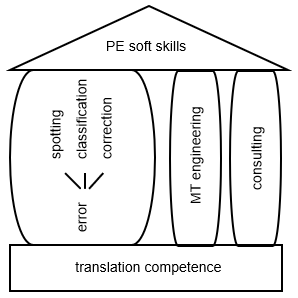
\includegraphics[height=0.4\textheight]{figures/Job Profile 1.PNG}
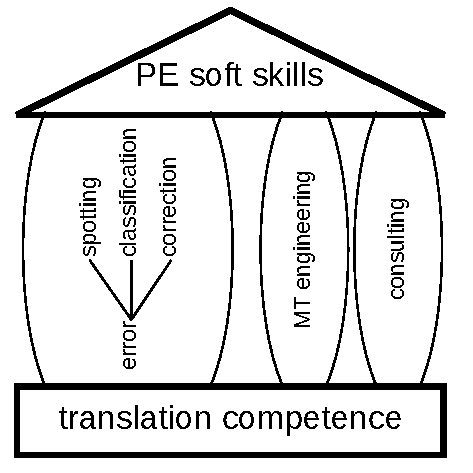
\includegraphics[height=0.4\textheight]{figures/jobprofile1.pdf}
\caption{PE competences for post-editors}
\label{fig:key:9:2:1}
\end{figure}


\subsection{PE competences for MT engineers}\label{sec:9:2:2}

A second job perspective might be called MT engineering (\figref{fig:key:9:2:2}). MT engineers are more focused on the technology. They have in-depth knowledge about how to train and maintain MT engines as well as deep knowledge of MT structures, and how to improve and evaluate the MT output. They are responsible for questions like what system is suitable for the job or for the company and what kind of data are needed for training. Further, they should have a lot of knowledge about (other) CAT tools like translation memory and terminology management systems, so that they can implement the technological support that best fits the respective project. To obtain these goals they also need basic knowledge on error handling and client consulting to be able to assess the post-editors needs and the project's requirements. Their risk assessment and service competences are an integral part of their job and can be judged as intermediate compared to the other job profiles.

\begin{figure} 
% 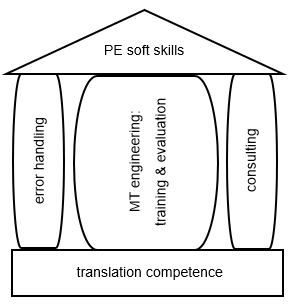
\includegraphics[height=0.4\textheight]{figures/Job Profile 2.PNG}
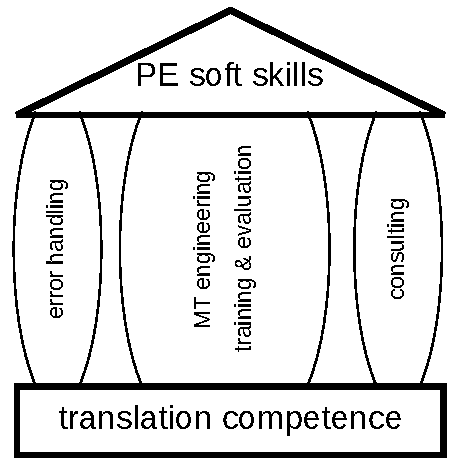
\includegraphics[height=0.4\textheight]{figures/jobprofile2.pdf}
\caption{PE competences for MT engineers}
\label{fig:key:9:2:2}
\end{figure}

\subsection{PE competences for PE consultants}\label{sec:9:2:3}

Finally, one job perspective for post-editors can be to work in a consulting position (\figref{fig:key:9:2:3}), where the main tasks are project and risk management, taking charge of the communication between the different stakeholders and making the decisions that are necessary to set up a PE project. For this, they naturally need basic knowledge on PE practice and MT engineering and they also must have profound knowledge about risk assessment and service, because they create the projects and decide which texts and projects can be post-edited and which not. They have to make decisions on the aspects we discussed in \sectref{sec:8}. Concerning the actors described in the ISO standard in section \sectref{sec:4}, PE consultants can also take the role of or work closely together with the translation service provider. 

\begin{figure} 
% 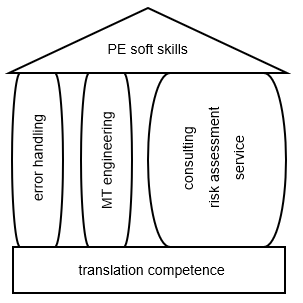
\includegraphics[height=0.4\textheight]{figures/Job Profile 3.PNG}
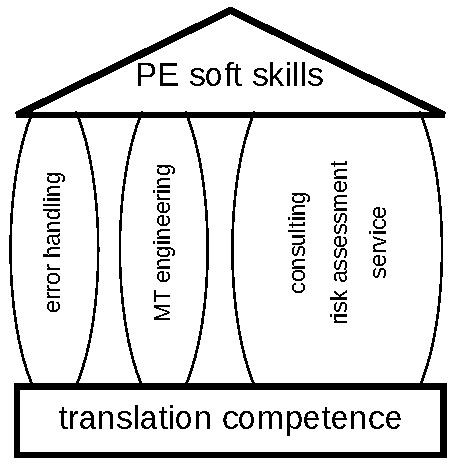
\includegraphics[height=0.4\textheight]{figures/jobprofile3.pdf}
\caption{PE competences for PE consultants}
\label{fig:key:9:2:3}
\end{figure}

\section{PE training and education}\label{sec:9:3}
\largerpage[2]
Training and education in PE should be in line with the different job profiles we described in \ref{sec:9:2}. As a prospective post-editor, you should specialise on the aspects of the job profile you are most interested in. 

If you do not have any translation experience and knowledge about translation studies at all, you should consider a translation university degree or a long term translation training to gain the relevant translation competences. When you choose a university/degree/programme, you might already keep in mind which job profile seems the most interesting for you and look at the curricula to see whether an institution offers PE courses, courses on MT or computational linguistics, and/or courses on project management.

If you are a professional translator, you have already gained a lot of PE knowledge in this book. You may want to look for courses on advanced training offered by universities or professional associations. The PE job profile is probably the closest to aim for if you want to build on your existing knowledge. Try to find a programme or some add-on courses that discuss practical aspects and offer some hands-on exercises. If you want to focus on MT engineering, you should try to gain some extra knowledge on the technology and might want to find some computer linguistic, MT, or artificial intelligence courses. If you want to focus on consulting, it would be advisable to gain some knowledge about project and risk management. Some PE practice would be helpful for the MT engineering and consulting profiles as well.

\newpage

\section*{Crossword puzzle -- chapter 9}

\begin{Puzzle}{15}{19}
|{}	|{}	|{}	|{}	|{}	|[6]P	|{}	|{}	|{}	|{}	|{}	|{}	|{}	|{}	|{}	|.
|{}	|{}	|{}	|{}	|{}	|S	|{}	|{}	|{}	|{}	|{}	|[1]T	|{}	|{}	|{}	|.
|{}	|{}	|{}	|{}	|{}	|Y	|{}	|[4]C	|{}	|{}	|{}	|R	|{}	|{}	|{}	|.
|{}	|{}	|{}	|{}	|{}	|C	|{}	|O	|{}	|{}	|{}	|A	|{}	|{}	|{}	|.
|[7]E	|R	|R	|O	|R	|H	|A	|N	|D	|L	|I	|N	|G	|{}	|{}	|.
|{}	|{}	|{}	|{}	|{}	|O	|{}	|S	|{}	|{}	|{}	|S	|{}	|{}	|{}	|.
|{}	|{}	|{}	|{}	|{}	|P	|{}	|U	|{}	|{}	|{}	|L	|{}	|{}	|{}	|.
|{}	|{}	|{}	|{}	|{}	|H	|{}	|L	|{}	|{}	|{}	|A	|{}	|{}	|{}	|.
|{}	|{}	|{}	|{}	|{}	|Y	|{}	|T	|{}	|{}	|{}	|T	|{}	|{}	|{}	|.
|{}	|{}	|{}	|{}	|{}	|S	|{}	|I	|{}	|{}	|{}	|I	|{}	|{}	|{}	|.
|{}	|{}	|{}	|{}	|{}	|I	|{}	|N	|{}	|{}	|{}	|O	|{}	|{}	|{}	|.
|{}	|{}	|{}	|{}	|{}	|O	|{}	|G	|{}	|{}	|{}	|N	|{}	|{}	|{}	|.
|{}	|{}	|{}	|{}	|{}	|L	|{}	|{}	|{}	|{}	|{}	|{}	|{}	|{}	|{}	|.
|{}	|{}	|{}	|{}	|{}	|O	|{}	|{}	|{}	|{}	|{}	|{}	|{}	|{}	|{}	|.
|{}	|{}	|{}	|[5]E	|N	|G	|I	|N	|E	|E	|R	|I	|N	|G	|{}	|.
|{}	|{}	|{}	|{}	|{}	|I	|{}	|{}	|{}	|{}	|{}	|{}	|{}	|{}	|{}	|.
|[3]C	|O	|R	|R	|E	|C	|T	|I	|O	|N	|{}	|{}	|{}	|{}	|{}	|.
|{}	|{}	|{}	|{}	|{}	|A	|{}	|{}	|{}	|{}	|{}	|{}	|{}	|{}	|{}	|.
|[2]E	|X	|T	|R	|A	|L	|I	|N	|G	|U	|I	|S	|T	|I	|C	|.
\end{Puzzle}

\begin{PuzzleClues}{\textbf{Across}}
\Clue{2}{EXTRALINGUISTIC}{What competence is needed for PE and translation from scratch that describes the knowledge about domain-specific contents, e.g. medical knowledge for translating and post-editing medical texts?}
\Clue{3}{CORRECTION}{What belongs to the error handling competence? Error spotting, error classification, and error ...}
\Clue{5}{ENGINEERING}{What do we call the competence that includes training and assessment of MT systems? MT ...}
\Clue{7}{ERRORHANDLING}{What is the most prominent competence pillar for the job profile of a post-editor?}
\end{PuzzleClues}

\begin{PuzzleClues}{\textbf{Down}}
\Clue{1}{TRANSLATION}{Which is one of the basic competences for post-editing?}
\Clue{4}{CONSULTING}{Which competence describes that post-editors must be able to inform clients about the pros and cons of using machine translation systems?}
\Clue{6}{PSYCHOPHYSIOLOGICAL}{The ability to concentrate and sustain attention, stress-resistance, logical reasoning, analytical thinking, quick-wittedness, an affinity for technologies are the ... components that are especially important for post-editors.}
\end{PuzzleClues}
